% ============================================================
% Capítulo III — Principio de Huygens
% Traducción de "Théorie mathématique de la lumière" (1889), cap. III
% Original: §§61-75, páginas 76-98
% ============================================================
\chapter{Principio de Huygens}
\label{cap:huygens}

\noindent\textbf{61.} El principio de Huygens, en el que se apoya la teoría
de la difracción, ha sido objeto de numerosas objeciones. Para disipar esas
objeciones y dar una justificación tan completa como sea posible de este
importante principio, nos veremos obligados a detenernos largamente en este
tema.

Expongamos primero las ideas de Huygens. Supongamos que, estando en reposo
todas las moléculas del éter, se da un ebranlement\footnote{Conservamos aquí
puntualmente el sentido físico del término francés \emph{ébranlement}: una
sacudida o perturbación inicial impartida a las moléculas del medio, origen
de la onda. En el resto del capítulo se traduce simplemente como
\emph{perturbación} o \emph{sacudida inicial}.} —una perturbación inicial—
a las contenidas en el interior de una esfera $A$ (figura~\ref{fig:cap3-1})
de radio muy pequeño, y que luego se abandona el éter a sí mismo. La
perturbación comunicada a las moléculas de $A$ se propagará en el éter;
Huygens admite que se produce una onda esférica, y que, al cabo de un tiempo
$t$, las únicas moléculas en movimiento ocupan una capa infinitamente
delgada situada en la superficie de una esfera $S$ de radio $Vt$,
concéntrica con $A$. Esta hipótesis equivale a admitir la posibilidad de
propagación de una onda aislada y, aunque experimentalmente la realización
de este hecho nunca tenga lugar, se puede usar esta abstracción en la
teoría. Siendo así, las únicas moléculas en movimiento al cabo del tiempo
$t+t'$ estarán situadas en una capa esférica $S'$ concéntrica con $S$ y de
radio $V(t+t')$.

\begin{enunciado}{Principio de Huygens}
El movimiento del éter en todo punto de la onda $S'$ es la resultante de
los movimientos que enviarían aisladamente todos los elementos de la misma
onda, considerada en una posición anterior $S$.
\end{enunciado}

Si este principio es cierto, debe poder deducirse de él que las moléculas en
movimiento al tiempo $t+t'$ están todas situadas en el interior de la capa
$S'$. Ahora bien, la onda parcial que proviene de la propagación del
movimiento que animaba, en el tiempo $t$, a un elemento $B$ de la onda $S$,
será una esfera de centro $B$ y radio $Vt'$; esa onda $s$ es, por tanto,
tangente a la onda $S'$. Lo mismo ocurrirá para todas las ondas parciales, y
se puede considerar la onda $S'$ como la envolvente de las ondas parciales
provenientes de los distintos puntos de $S$. Resulta entonces evidente que
no podrá haber movimiento más allá de la onda $S'$. Pero nada prueba
\emph{a priori} que no lo haya más acá. A primera vista, incluso parece
difícil que así sea, pues los movimientos de las moléculas de la esfera de
perturbación, al parecer tener el mismo sentido, deberían dar origen a
movimientos del mismo sentido que no pueden destruirse. Huygens explicaba
esta anomalía admitiendo que, siendo la capa $S$ infinitamente delgada, los
movimientos provenientes de la perturbación de los distintos elementos de
esa superficie debían ser infinitamente pequeños, y que solo podían ser
apreciables en la superficie $S'$, donde se componen un gran número de esos
movimientos. Esta explicación no resiste un análisis riguroso.

\begin{figure}[h]
\centering
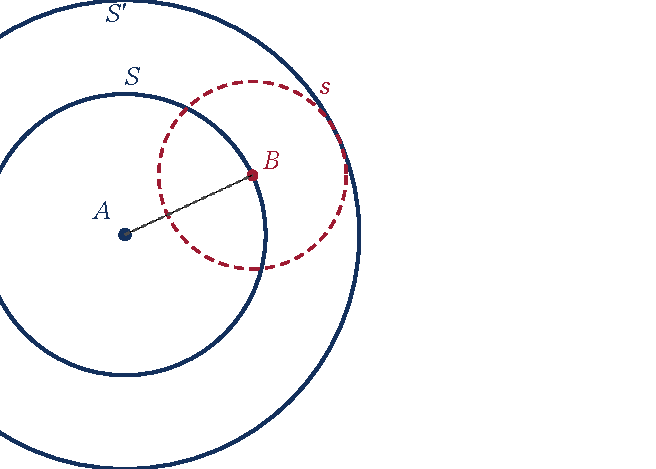
\includegraphics[width=0.85\textwidth]{figuras/pdf/cap03-fig1.pdf}
\caption{Esquema de Huygens: la perturbación inicial en la esfera $A$ se
propaga como onda esférica $S$, y luego como $S'$.}
\label{fig:cap3-1}
\end{figure}

\noindent\textbf{62.} Fresnel, en su teoría de la difracción, modifica el
principio de Huygens al considerar, ya no una onda aislada, sino una
sucesión de ondas provenientes de movimientos vibratorios. Así enuncia él
mismo este principio:

\begin{enunciado}{Principio de Huygens-Fresnel}
Las vibraciones de una onda luminosa en cada uno de sus puntos pueden
considerarse como la suma de los movimientos elementales que enviarían en
ese mismo instante, actuando aisladamente, todas las partes de esa onda
consideradas en cualquiera de sus posiciones anteriores.
\end{enunciado}

A este enunciado añade Fresnel, en nota: «Considero siempre la
sucesión de una infinidad de ondulaciones, o una vibración general del
fluido. Solo en ese sentido puede decirse que dos ondas luminosas se
destruyen cuando están a media ondulación una de otra. Las fórmulas de
interferencia que acabo de dar no son aplicables al caso de una ondulación
aislada, que por lo demás no es el de la naturaleza.»\footnote{\emph{Œuvres
de Fresnel}, t.~I, p.~293.} Al considerar así ondas sucesivas, los
movimientos de las moléculas de $S$ son unas veces en un sentido, otras en
el contrario, y puede concebirse que, al tiempo $t+t'$, las moléculas que
quedan fuera de la superficie $S'$ no estén en movimiento. Esta explicación
dista de estar libre de todo reproche, como veremos en el párrafo
siguiente. Por lo demás, la teoría de la propagación de una onda aislada
—propagación matemáticamente posible— deja subsistir una dificultad que es
necesario explicar.

\noindent\textbf{63. Controversia de Fresnel con Poisson.} — Ya se
considere una onda aislada o una serie de ondas sucesivas, el principio de
Huygens lleva a admitir que, además de la onda $S'$, se produce otra, $S''$,
que es la envolvente interior de las ondas elementales $s$. Esta es una de
las objeciones que Poisson hace a Fresnel, en una carta\footnote{\emph{Œuvres
de Fresnel}, t.~II, p.~209.} de la que extraemos el siguiente pasaje:
«También le haré notar que, en el razonamiento que lo conduce a la fórmula
de la página 287 de su Memoria sobre la difracción\footnote{Es la fórmula
$\left[\left(\int ds\cos\!\left(\pi\dfrac{s^2(a+b)}{ab\lambda}\right)\right)^2
+\left(\int ds\sin\!\left(\pi\dfrac{s^2(a+b)}{ab\lambda}\right)\right)^2\right]^{1/2}$,
que da la velocidad del desplazamiento en el punto $P$ y que Fresnel obtuvo
apoyándose en el principio de Huygens (\emph{Œuvres de Fresnel}, t.~I,
p.~316). $a$ designa la distancia $CM$, $b$ la distancia $MP$.}, nada
expresa que el punto $P$ (figura~\ref{fig:cap3-2}) esté situado más allá de
la onda $AMF$, y que, si estuviera situado más acá de esa onda, el mismo
razonamiento, aplicado palabra por palabra, lo conduciría a una fórmula
semejante para expresar la velocidad que recibe, con la única diferencia de
que, en lugar de $a+b$, esa fórmula contendría $a-b$, que sería entonces la
distancia $CP$. De sus principios se seguiría, pues, que la onda $AMF$,
incluso cuando está completa, debería producir movimiento tanto más acá como
más allá de su posición, conclusión que bastaría para mostrar que hay algún
vicio en su manera de plantear la cuestión. Y, en efecto, la producción de
una onda nueva por delante de la que usted considera, y la no comunicación
del movimiento hacia atrás, solo se dan en razón de una relación
determinada que subsiste, en la onda dada, entre las condensaciones y las
velocidades propias de las moléculas fluidas, y de ningún modo en razón de
la interferencia de las ondas elementales originadas en todos sus puntos en
instantes distintos.»

\begin{figure}[h]
\centering
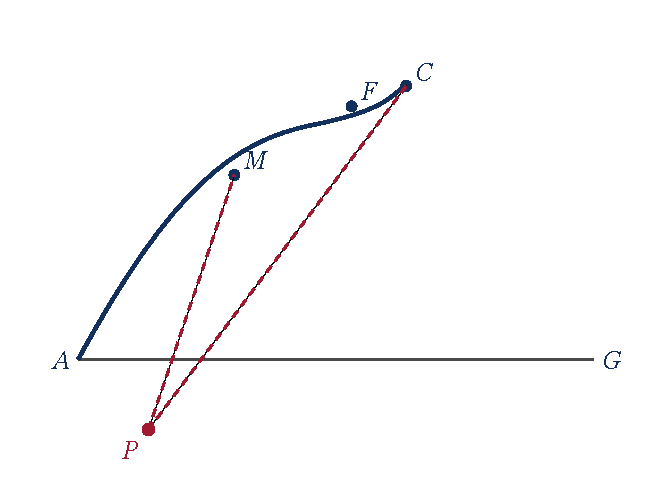
\includegraphics[width=0.85\textwidth]{figuras/pdf/cap03-fig2.pdf}
\caption{Diagrama de la carta de Poisson a Fresnel: el punto $P$ y la onda
$AMF$.}
\label{fig:cap3-2}
\end{figure}

\noindent\textbf{64.} En su respuesta a esta carta, Fresnel, tras contestar
a otras objeciones de Poisson, llega por fin a la verdadera explicación de
la anomalía que tanto tiempo había detenido a los geómetras. Hay, dice,
dos cosas que considerar en el movimiento de una molécula: la velocidad de
la que está animada y su alejamiento de su posición de equilibrio; de ahí
resultan dos sistemas de ondas derivadas.

Pero, antes de citar ese pasaje de Fresnel, debemos dar algunas
explicaciones sobre lo que él llama \emph{la ley del coseno}. En la época
de esta controversia, Fresnel ya había hecho su gran descubrimiento de la
transversalidad de las vibraciones. Pero Poisson y los geómetras de su
tiempo se negaban a admitirlo. Así, Fresnel, deseoso de reducir la
divergencia de sus puntos de vista con los de Poisson, y convencido de que
su teoría de la difracción era igualmente aplicable a todas las hipótesis,
razona constantemente como si las vibraciones fueran longitudinales.

Así llega, mediante un razonamiento que por lo demás no estaría libre de
todo reproche, a esta consecuencia: que el movimiento enviado por un punto
$B$ (figura~\ref{fig:cap3-3}) de la onda $S$ a un punto $D$ de la onda $S'$
es proporcional al coseno del ángulo $DBC$ formado por la dirección $DB$
con la normal a la onda $S$. Este razonamiento no es en absoluto aplicable
al caso de los movimientos transversales.

Por fortuna, la ley del coseno no desempeña ningún papel esencial en la
teoría de Fresnel, y debe considerarse solo como un incidente de su
controversia. Las objeciones a las que esta ley pueda dar lugar no afectan
en nada a la teoría misma.

\begin{figure}[h]
\centering
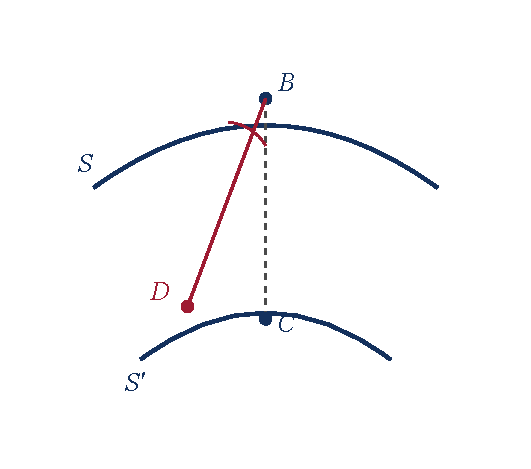
\includegraphics[width=0.7\textwidth]{figuras/pdf/cap03-fig3.pdf}
\caption{La ``ley del coseno'' de Fresnel: ángulo $DBC$ entre $DB$ y la
normal a la onda $S$.}
\label{fig:cap3-3}
\end{figure}

\noindent\textbf{65.} Citemos ahora el pasaje más importante de la carta de
Fresnel (\emph{Œuvres complètes}, t.~II, p.~227).

\begin{quote}
«Usted objetará quizá todavía al razonamiento que acabo de hacer para el
caso de una pequeña perturbación, que establecería la existencia de rayos
de igual intensidad en sentido opuesto, incluso cuando la perturbación
inicial formara parte de una onda derivada; pero responderé, como ya lo he
hecho, que esto no es en absoluto una consecuencia del principio en el que
me apoyo. En efecto, llego a esta ley del coseno considerando por separado
la onda producida por las velocidades impresas a las moléculas comprendidas
en el centro de perturbación, y la que resulta de sus simples
desplazamientos, para luego sumarlas: ahora bien, cuando estas dos ondas
empujan el fluido en el mismo sentido, se refuerzan mutuamente por
superposición; y si las intensidades de los distintos puntos de la
superficie siguen la ley del coseno en una y en otra, esa misma ley se dará
también en la onda resultante de su reunión. Si tienden a empujar las
moléculas del fluido en sentidos opuestos, las velocidades absolutas que
aportan se restan, y pueden incluso destruirse mutuamente, en el caso de
que sean iguales; esto es lo que ocurre con las ondas retrógradas, cuando
el centro de perturbación tiene la constitución particular de las ondas
derivadas. Considérese, por ejemplo, un elemento de una onda de este tipo
en el momento en que sus moléculas son empujadas hacia adelante, es decir,
en el sentido de propagación de la onda derivada: se sabe que entonces ese
movimiento hacia adelante va acompañado de una condensación, es decir, de
un acercamiento de las moléculas; si las moléculas estuvieran solo
desplazadas y, por lo demás, sin velocidad en ese mismo instante, de su
acercamiento resultaría una fuerza expansiva que empujaría el fluido tanto
hacia atrás como hacia adelante, y produciría así una onda retrógrada
semejante a la que excitaría hacia adelante, pero en la que las velocidades
absolutas serían de signo contrario; si, por otro lado, las moléculas se
encontraran en sus posiciones de equilibrio en el momento en que se
considera la perturbación, y recibieran solo en ese instante las
velocidades que las empujan hacia adelante, resultaría también de ello una
onda hacia atrás, igual que una onda hacia adelante, puesto que esas
moléculas serían seguidas por las que están detrás, y así sucesivamente;
la onda retrógrada tendría todavía la misma intensidad que la onda que se
propagaría hacia adelante, y desplazaría las moléculas del fluido en el
mismo sentido; pero la onda retrógrada resultante de la simple condensación
las empuja en sentido contrario. Estos dos movimientos se restarán,
entonces, el uno del otro en las ondas retrógradas debidas a la
condensación y a las velocidades de las moléculas, mientras que se sumarán
en las dos ondas que se propagan hacia adelante; si, pues, estas dos causas
tienden a producir efectos iguales, como ocurre en el caso particular de
las ondas derivadas, las ondas retrógradas se borrarán mutuamente, y las
vibraciones solo podrán propagarse en el sentido de la marcha de la onda
derivada.»
\end{quote}

Esa era, en efecto, la verdadera explicación del principio de Huygens;
vamos a mostrarla con mayor rigor en lo que sigue.

\section{Integración de las ecuaciones de los movimientos transversales en
el caso de las ondas esféricas}

\noindent\textbf{66.} Retomemos las ecuaciones de los movimientos
transversales
\[
\frac{d^2\xi}{dt^2}=V^2\Delta\xi,\qquad
\frac{d^2\eta}{dt^2}=V^2\Delta\eta,\qquad
\frac{d^2\zeta}{dt^2}=V^2\Delta\zeta,
\]
que ya resolvimos para el caso de las ondas planas (§50), y propongámonos hallar
sus integrales en el caso de las ondas esféricas.

En las ondas de esta naturaleza, los desplazamientos y las velocidades de
un punto $M$ (figura~\ref{fig:cap3-4}) deben tener los mismos valores para
todos los puntos situados a una misma distancia $r$ del centro de las
ondas; luego $\xi,\eta,\zeta$ y sus derivadas dependerán únicamente de $r$ y
del tiempo $t$. Tomando como origen de coordenadas el centro de las ondas
esféricas y llamando $x,y,z$ a las coordenadas del punto $M$, tendremos
\[
r^2=x^2+y^2+z^2.
\]
Pongamos
\[
\xi=\frac{u}{r},
\]
siendo $u$ una función cualquiera de $r$ y de $t$, y busquemos cuál debe ser
la forma de esta función para que satisfaga las ecuaciones del movimiento.

La cantidad $\Delta\xi$ es una función lineal y homogénea de $u$ y de sus
dos primeras derivadas respecto de $r$; podemos escribirla
\[
\Delta\xi = Au + B\frac{du}{dr} + C\frac{d^2u}{dr^2}.
\]

\begin{figure}[h]
\centering
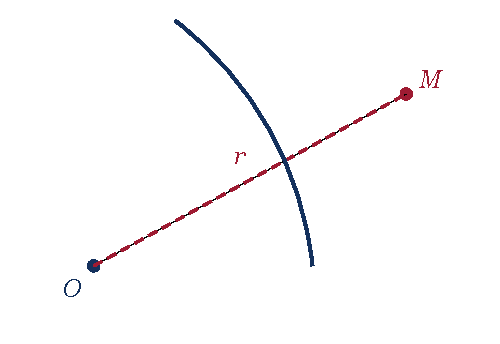
\includegraphics[width=0.85\textwidth]{figuras/pdf/cap03-fig4.pdf}
\caption{Onda esférica de centro $O$: el punto $M$ a distancia $r$.}
\label{fig:cap3-4}
\end{figure}

\noindent\textbf{67.} El valor de los coeficientes $A,B,C$ podría obtenerse
calculando las derivadas segundas de $\xi$ respecto de $x,y,z$ y
sumándolas, pero resulta más simple determinarlos haciendo hipótesis
particulares sobre la función $u$.

Supongamos primero que $u=1$; entonces $\xi=1/r$. Es la forma de la función
potencial en la atracción de dos puntos según la ley de Newton. Debe
tenerse entonces $\Delta\xi=0$, y como la expresión de $\Delta\xi$ se
reduce a $A$ en este caso particular, $A$ debe ser nulo.

Tomemos $u=r$; tendremos $\xi=1$, y por tanto $\Delta\xi=0$. Por otra
parte, tenemos $du/dr=1$, $d^2u/dr^2=0$; por consiguiente, como $A$ es nulo
según lo anterior,
\[
\Delta\xi = B\,\frac{du}{dr} = 0.
\]
El coeficiente $B$ debe ser, entonces, también nulo.

Para hallar el coeficiente $C$, hagamos $u=r^3$; la derivada segunda de
esta función respecto de $r$ será igual a $6r$, y el valor de $\Delta\xi$
se reducirá a $\Delta\xi=6Cr$. Pero si $u=r^3$, tenemos
$\xi=r^2=x^2+y^2+z^2$, y el cálculo da para $\Delta\xi$: $\Delta\xi=6$.
Igualando estos dos valores de $\Delta\xi$, obtenemos para $C$:
$C=1/r$.

La expresión de $\Delta\xi$ en el caso general es, por tanto,
\[
\Delta\xi = \frac{1}{r}\frac{d^2u}{dr^2}.
\]

Sustituyendo este valor en la primera de las ecuaciones del movimiento y
reemplazando $d^2\xi/dt^2$ por su valor $\frac{1}{r}\dfrac{d^2u}{dt^2}$,
obtendremos una ecuación que determinará $u$; esta ecuación es
\[
\frac{1}{r}\frac{d^2u}{dt^2} = V^2\frac{1}{r}\frac{d^2u}{dr^2},
\]
o bien
\[
\frac{d^2u}{dt^2} = V^2\frac{d^2u}{dr^2}.
\]
Integrando, se obtiene
\[
u = F(r-Vt) + F_1(r+Vt),
\]
de donde
\[
\xi = \frac{F(r-Vt)}{r} + \frac{F_1(r+Vt)}{r}.
\]

\noindent\textbf{68.} Siendo $F$ y $F_1$ funciones arbitrarias, podemos
suponer que una de ellas, $F_1$, se reduzca a $0$; tendremos entonces
\[
\xi = \frac{F(r-Vt)}{r},
\]
expresión que satisface las ecuaciones del movimiento. Por consiguiente, en
el caso general, $\xi$ puede considerarse como el desplazamiento resultante
de dos movimientos que se propagan por ondas esféricas a partir del centro
$O$, uno con velocidad $V$, el otro con velocidad $-V$. El factor $1/r$ que
aparece en la expresión de $\xi$ muestra que el movimiento se debilita a
medida que nos alejamos del centro de la perturbación.

Las dos últimas ecuaciones de los movimientos transversales darían, para
$\eta$ y $\zeta$, expresiones análogas a la que acabamos de hallar para
$\xi$.

\noindent\textbf{69.} Cuando se dan los valores iniciales de las
componentes de las velocidades, el movimiento queda completamente
determinado y se pueden hallar las funciones $F$ y $F_1$. Supongamos que en
el tiempo $t=0$ tenemos
\[
\xi=\varphi(r),\qquad \frac{d\xi}{dt}=\psi(r).
\]
Haciendo $t=0$ en la expresión de $\xi$, e igualando al valor dado
$\varphi(r)$, obtenemos la relación
\[
r\varphi(r) = F(r) + F_1(r). \tag{1}
\]
La derivada de $\xi$ respecto del tiempo es
\[
\frac{d\xi}{dt} = -V\frac{F'(r-Vt)}{r} + V\frac{F_1'(r+Vt)}{r};
\]
su valor para $t=0$ se reduce a
\[
\frac{d\xi}{dt} = -V\frac{F'(r)}{r} + V\frac{F_1'(r)}{r}.
\]
Tenemos, entonces, la relación
\[
r\psi(r) = V\bigl(F_1'-F'\bigr). \tag{2}
\]
Las relaciones (1) y (2) determinarán las funciones $F$ y $F_1$.

Una solución particular de las ecuaciones de los movimientos transversales
que resulta interesante en óptica es aquella en la que se tiene
\[
F_1(r)=0,\qquad F(r)=e^{-i\alpha r}.
\]
El valor de $\xi$ es entonces
\[
\xi = \frac{e^{-i\alpha(r-Vt)}}{r}.
\]
Su derivada segunda respecto de $t$ vale $-\alpha^2V^2\xi$.\footnote{El
original impreso dice «a pour valeur $\alpha^2V^2\xi$», omitiendo el signo
menos, que sin embargo sí aparece en la línea siguiente. En efecto,
$\frac{d}{dt}e^{-i\alpha(r-Vt)}=i\alpha V\,e^{-i\alpha(r-Vt)}$, y derivando
otra vez se obtiene el factor $(i\alpha V)^2=-\alpha^2V^2$.} Como $\xi$
satisface las ecuaciones del movimiento, debe cumplirse
\[
\frac{d^2\xi}{dt^2}=V^2\Delta\xi,\qquad
-\alpha^2V^2\xi = V^2\Delta\xi,
\]
o, finalmente,
\[
\Delta\xi + \alpha^2\xi = 0.
\]

\section{Integrales generales de las ecuaciones de los movimientos
transversales}

\noindent\textbf{70.} Consideremos la primera de estas ecuaciones, que
escribiremos en la forma
\[
\frac{d^2\xi}{dt^2}=V^2\Delta\xi. \tag{1}
\]
Tendremos la integral general de esta ecuación si encontramos una función
$\xi$ de $x,y,z$ y $t$ que la satisfaga idénticamente y que se reduzca,
para $t=0$, a una función arbitraria de $x,y,z$, mientras que su derivada
$d\xi/dt$ se reduzca también, para $t=0$, a otra función arbitraria de
$x,y,z$. La integral general contiene, pues, dos funciones arbitrarias.

Veamos primero a qué nos conduce la aplicación del principio de Huygens.
Supongamos que, en el origen de los tiempos, todas las moléculas del éter
estén perturbadas de tal modo que la perturbación inicial en el punto
$x',y',z'$ sea igual a $F(x',y',z')$. Al cabo del tiempo $t$, el punto
$x',y',z'$ habrá enviado una perturbación igual a $F/r$ a todos los puntos
$x,y,z$ situados a una distancia $r=Vt$ del punto $x',y',z'$, y no habrá
enviado ninguna a los puntos situados a una distancia mayor o menor.

Luego, según el principio de Huygens, el punto $x,y,z$ habrá recibido en el
instante $t$ una perturbación $F/r$ de todos los puntos $x',y',z'$ de la
esfera que tiene por centro $x,y,z$ y por radio $r=Vt$, y no habrá recibido
ninguna de ningún otro punto del espacio.

Pongamos, pues,
\[
\xi = \int \frac{F(x',y',z')}{r}\,d\omega, \tag{2}
\]
extendiéndose la integral a todos los elementos $d\omega$ de la esfera de
centro $x,y,z$ y radio $r=Vt$, y designando $x',y',z'$ las coordenadas del
elemento $d\omega$. El valor de la integral dependerá evidentemente del
centro y del radio de esta esfera, y por consiguiente $\xi$ será función de
$x,y,z$ y de $t$. Debemos, pues, para justificar el principio de Huygens,
demostrar que el valor (2) de $\xi$ satisface la ecuación (1).

Calculemos $d\xi/dx$. Para ello, demos a $x$ un
incremento $dx$ conservando $y$, $z$, $t$ —y por consiguiente $r$— sus
valores; esto equivale a dar a la esfera una traslación $dx$ paralela al
eje $x$. De ello resultará, para $x'$, un incremento $dx$, mientras que
$y'$, $z'$, $d\omega$ y $r$ conservarán el mismo valor. El incremento de
$F(x',y',z')$ será $\dfrac{dF}{dx'}dx$, y tendremos
\[
d\xi = \int \frac{dF}{dx'}\,\frac{dx\,d\omega}{r}.
\]
Como el incremento de $x'$ es el mismo para todos los elementos de la
integral, podemos sacar $dx$ como factor, y dividiendo ambos miembros de la
igualdad por esta cantidad, obtenemos
\[
\frac{d\xi}{dx} = \int \frac{dF}{dx'}\,\frac{d\omega}{r}.
\]
Derivando una segunda vez respecto de $x$, obtenemos, para la derivada
segunda,
\[
\frac{d^2\xi}{dx^2} = \int \frac{d^2F}{dx'^2}\,\frac{d\omega}{r}.
\]
El mismo razonamiento conduciría a las expresiones
\[
\frac{d^2\xi}{dy^2} = \int \frac{d^2F}{dy'^2}\,\frac{d\omega}{r},\qquad
\frac{d^2\xi}{dz^2} = \int \frac{d^2F}{dz'^2}\,\frac{d\omega}{r},
\]
para las derivadas segundas de $\xi$ respecto de $y$ y de $z$. Sumando
estas derivadas segundas, obtenemos
\[
\Delta\xi = \int \Delta F(x',y',z')\,\frac{d\omega}{r}. \tag{3}
\]

\noindent\textbf{71.} Busquemos ahora la derivada segunda de la integral
(2) respecto del tiempo. Si damos al tiempo $t$ un incremento $dt$ sin
variar $x,y,z$, el centro de la esfera no cambiará, pero su radio sufrirá
un incremento
\[
dr = V\,dt.
\]
El elemento de superficie $d\omega$ se convertirá en $d\omega'$. Podemos
hacer desaparecer $d\omega$ de la integral introduciendo el ángulo sólido
$d\sigma$ bajo el cual se ve este elemento desde el centro de la esfera; se
tiene
\[
d\omega = r^2\,d\sigma,\qquad\text{de donde}\qquad \frac{d\omega}{r}=r\,d\sigma.
\]
Por consiguiente, la integral se convierte en
\[
\xi = \int F(x',y',z')\,r\,d\sigma, \tag{4}
\]
y como $r$ es el mismo para todos los elementos de la integral, podemos
escribir
\[
\xi = r\int F(x',y',z')\,d\sigma.
\]

Si, pues, $r$ sufre un incremento $dr$, el incremento $d\xi$ que de ello
resultará para $\xi$ será\footnote{El original impreso dice
«$d\xi = dr\int F\,d\sigma = r\,d.\!\int F\,d\sigma$», con un signo $=$ en
lugar de $+$: es una errata evidente, pues se trata simplemente de la regla
del producto aplicada a $r\cdot\int F\,d\sigma$, como confirma la línea
siguiente.}
\[
d\xi = dr\int F\,d\sigma + r\,d\!\int F\,d\sigma,
\]
o bien
\[
d\xi = dr\int F\,d\sigma + r\,dr\int \frac{dF}{dr}\,d\sigma.
\]

Para calcular el valor de la segunda integral que entra en esta expresión,
observemos que, siendo el radio $r$ normal al elemento de superficie
$d\omega$, se tiene, según el teorema de Green,
\[
\int \frac{dF}{dr}\,d\omega = \int \Delta F\,d\tau,
\]
siendo $d\tau$ un elemento de volumen, y extendiéndose la integral del
segundo miembro a toda la esfera. Introduciendo en esta última igualdad el
ángulo sólido $d\sigma$ que corresponde a $d\omega$, se convierte en
\[
\int \frac{dF}{dr}\,d\sigma = \frac{1}{r^2}\int \Delta F\,d\tau. \tag{5}
\]

Podemos, pues, reemplazar el valor hallado antes para $d\xi$ por el
siguiente:
\[
d\xi = dr\int F\,d\sigma + \frac{dr}{r}\int \Delta F\,d\tau;
\]
o, dividiendo por $dr=V\,dt$,
\[
\frac{1}{V}\frac{d\xi}{dt} = \int F\,d\sigma + \frac{1}{r}\int \Delta F\,d\tau. \tag{6}
\]
Diferenciando esta última expresión respecto de $r$, obtenemos la igualdad
\[
\frac{1}{V^2}\frac{d^2\xi}{dt^2} = \int \frac{dF}{dr}\,d\sigma -
\frac{1}{r^2}\int \Delta F\,d\tau + \frac{1}{r}\frac{d}{dr}\cdot\int \Delta F\,d\tau,
\]
que, teniendo en cuenta la relación (5), se reduce a
\[
\frac{1}{V^2}\frac{d^2\xi}{dt^2} = \frac{1}{r}\frac{d}{dr}\cdot\int \Delta F\,d\tau. \tag{7}
\]

El segundo miembro de esta relación es, salvo el factor $\dfrac{1}{r\,dr}$,
el valor de la integral $\int \Delta F\,d\tau$ extendida a los elementos de
volumen de una capa comprendida entre las esferas de radios $r$ y $r+dr$.
Consideremos uno de estos elementos, limitado por esas dos esferas y por un
cono que tiene por vértice el centro común de ambas esferas y por base el
elemento $d\omega$ de la superficie de la primera esfera. El volumen de
este elemento será, despreciando los infinitésimos de orden superior al
tercero, $d\omega\,dr$. Por consiguiente, la integral anterior se convierte
en
\[
\int \Delta F\,d\omega\,dr,\qquad\text{o bien}\qquad dr\int \Delta F\,d\omega,
\]
integral extendida a todos los elementos de la esfera de radio $r$. Se
obtiene entonces, para la relación (7),
\[
\frac{1}{V^2}\frac{d^2\xi}{dt^2} = \frac{1}{r}\int \Delta F\,d\omega. \tag{8}
\]

\begin{calculodetallado}[: de la ecuación (4) a las ecuaciones (5)--(8)]
En todo este pasaje el punto $(x,y,z)$ está fijo y solo varía el tiempo
$t$, y con él el radio $r=Vt$. Igual que Poincaré, escribimos $d/dr$, $d/dt$
para las derivadas parciales. Conviene describir cada punto de la esfera
mediante su dirección: si $\mathbf{n}=(n_1,n_2,n_3)$ es un vector unitario,
el punto de la esfera de centro $(x,y,z)$ y radio $r$ en esa dirección es
\[
(x',y',z') = (x+rn_1,\; y+rn_2,\; z+rn_3).
\]
El ángulo sólido $d\sigma$ es el elemento de área de la esfera
\emph{unidad} de direcciones $\mathbf{n}$: no depende de $r$, y el dominio
de integración (todas las direcciones, de área total $4\pi$) tampoco. Esta
es la razón de reemplazar $d\omega$ por $d\sigma$: en
$\xi = r\int F\,d\sigma$, toda la dependencia en $r$ está en el factor $r$
y dentro del integrando.

\medskip
\noindent\textbf{Paso 0: la expresión de $d\xi$.}
Por la regla del producto,
\[
\frac{d\xi}{dr} = \frac{d}{dr}\Bigl(r\int F\,d\sigma\Bigr)
= \int F\,d\sigma + r\,\frac{d}{dr}\int F\,d\sigma .
\]
Como el dominio de integración en $\mathbf{n}$ no depende de $r$, la
derivada entra bajo el signo integral:
$\dfrac{d}{dr}\displaystyle\int F\,d\sigma = \int \dfrac{dF}{dr}\,d\sigma$,
donde, por la regla de la cadena,
\[
\frac{dF}{dr} = \frac{d}{dr}F(x+rn_1,\,y+rn_2,\,z+rn_3)
= \frac{dF}{dx'}\,n_1 + \frac{dF}{dy'}\,n_2 + \frac{dF}{dz'}\,n_3
= \nabla F\cdot\mathbf{n}.
\]
Multiplicando por $dr$:
$d\xi = dr\displaystyle\int F\,d\sigma + r\,dr\int \frac{dF}{dr}\,d\sigma$.

\medskip
\noindent\textbf{Paso 1: el teorema de Green que se usa.}
Lo que Poincaré llama «teorema de Green» es aquí el teorema de la
divergencia (de Gauss--Ostrogradski): si $B$ es la bola de centro
$(x,y,z)$ y radio $r$, $S$ su esfera frontera y $\mathbf{n}$ la normal
unitaria exterior a $S$, para todo campo vectorial $\mathbf{G}$ con
derivadas continuas se tiene
\[
\int_B \nabla\cdot\mathbf{G}\;d\tau = \int_S \mathbf{G}\cdot\mathbf{n}\;d\omega .
\]
Apliquémoslo al campo $\mathbf{G}=\nabla F
=\bigl(\tfrac{dF}{dx'},\tfrac{dF}{dy'},\tfrac{dF}{dz'}\bigr)$ (suponemos $F$
con derivadas segundas continuas). Su divergencia es
\[
\nabla\cdot\nabla F = \frac{d^2F}{dx'^2}+\frac{d^2F}{dy'^2}+\frac{d^2F}{dz'^2}
= \Delta F,
\]
y su componente normal es la derivada normal
$\nabla F\cdot\mathbf{n} = \dfrac{\partial F}{\partial n}$. Por tanto
\[
\int_S \frac{\partial F}{\partial n}\,d\omega = \int_B \Delta F\,d\tau .
\]
Ahora bien, en una esfera la normal exterior en cada punto tiene
precisamente la dirección del radio que va del centro a ese punto: es el
mismo vector $\mathbf{n}$ que usamos para parametrizar la esfera. Esto es
lo que significa «el radio $r$ es normal al elemento $d\omega$». En
consecuencia, por el Paso 0,
\[
\frac{dF}{dr} = \nabla F\cdot\mathbf{n} = \frac{\partial F}{\partial n},
\]
y el teorema toma la forma que usa Poincaré:
\[
\int \frac{dF}{dr}\,d\omega = \int \Delta F\,d\tau,
\]
con la integral de la izquierda sobre la superficie de la esfera de radio
$r$ y la de la derecha sobre todo su volumen.

\medskip
\noindent\textbf{Paso 2: la relación (5).}
Sobre la esfera de radio $r$ se tiene $d\omega = r^2\,d\sigma$, y $r^2$ es
el mismo para todos los elementos, así que sale de la integral:
\[
\int \frac{dF}{dr}\,d\omega = \int \frac{dF}{dr}\,r^2\,d\sigma
= r^2\int \frac{dF}{dr}\,d\sigma .
\]
Igualando con el Paso 1,
\[
r^2\int \frac{dF}{dr}\,d\sigma = \int \Delta F\,d\tau,
\qquad\text{es decir,}\qquad
\int \frac{dF}{dr}\,d\sigma = \frac{1}{r^2}\int \Delta F\,d\tau, \tag{5}
\]
que es la relación (5).

\medskip
\noindent\textbf{Paso 3: la relación (6).}
Sustituimos (5) en el segundo término de $d\xi$ (Paso 0):
\[
r\,dr\int \frac{dF}{dr}\,d\sigma
= r\,dr\cdot\frac{1}{r^2}\int \Delta F\,d\tau
= \frac{dr}{r}\int \Delta F\,d\tau,
\]
de modo que
\[
d\xi = dr\int F\,d\sigma + \frac{dr}{r}\int \Delta F\,d\tau .
\]
Este incremento $d\xi$ es el que produce un incremento $dt$ del tiempo
(con $x,y,z$ fijos), y $dr = V\,dt$. Dividiendo ambos miembros por $dr$:
\[
\frac{d\xi}{dr} = \int F\,d\sigma + \frac{1}{r}\int \Delta F\,d\tau ,
\]
y como
$\dfrac{d\xi}{dr} = \dfrac{d\xi}{V\,dt} = \dfrac{1}{V}\dfrac{d\xi}{dt}$,
\[
\frac{1}{V}\frac{d\xi}{dt} = \int F\,d\sigma + \frac{1}{r}\int \Delta F\,d\tau . \tag{6}
\]

\medskip
\noindent\textbf{Paso 4: la relación (7).}
Derivamos (6) respecto de $r$, término a término.

\emph{Primer miembro.} Como $r=Vt$, derivar respecto de $r$ es lo mismo
que derivar respecto de $t$ y dividir por $V$:
$\dfrac{d}{dr} = \dfrac{1}{V}\dfrac{d}{dt}$. Luego
\[
\frac{d}{dr}\Bigl(\frac{1}{V}\frac{d\xi}{dt}\Bigr)
= \frac{1}{V}\frac{d}{dt}\Bigl(\frac{1}{V}\frac{d\xi}{dt}\Bigr)
= \frac{1}{V^2}\frac{d^2\xi}{dt^2}.
\]

\emph{Primer término del segundo miembro.} Por el mismo argumento del
Paso 0,
\[
\frac{d}{dr}\int F\,d\sigma = \int \frac{dF}{dr}\,d\sigma .
\]

\emph{Segundo término del segundo miembro.} Llamemos
$I(r)=\int \Delta F\,d\tau$ a la integral sobre la bola de radio $r$; es
una función de $r$, porque la bola crece con $r$. El término es el
producto $\frac{1}{r}\cdot I(r)$, y por la regla del producto, usando
$\frac{d}{dr}\bigl(\frac{1}{r}\bigr)=-\frac{1}{r^2}$,
\[
\frac{d}{dr}\Bigl(\frac{1}{r}\,I(r)\Bigr)
= -\frac{1}{r^2}\,I(r) + \frac{1}{r}\,\frac{dI}{dr}
= -\frac{1}{r^2}\int \Delta F\,d\tau + \frac{1}{r}\frac{d}{dr}\int \Delta F\,d\tau .
\]

Reuniendo los tres resultados,
\[
\frac{1}{V^2}\frac{d^2\xi}{dt^2}
= \int \frac{dF}{dr}\,d\sigma
- \frac{1}{r^2}\int \Delta F\,d\tau
+ \frac{1}{r}\frac{d}{dr}\int \Delta F\,d\tau .
\]
Por (5), el primer término vale exactamente
$\frac{1}{r^2}\int \Delta F\,d\tau$, de modo que los dos primeros términos
se cancelan:
\[
\int \frac{dF}{dr}\,d\sigma - \frac{1}{r^2}\int \Delta F\,d\tau
= \frac{1}{r^2}\int \Delta F\,d\tau - \frac{1}{r^2}\int \Delta F\,d\tau = 0,
\]
y queda
\[
\frac{1}{V^2}\frac{d^2\xi}{dt^2} = \frac{1}{r}\frac{d}{dr}\int \Delta F\,d\tau . \tag{7}
\]

\medskip
\noindent\textbf{Paso 5: de (7) a (8), la capa esférica.}
Escribamos la derivada como cociente de incrementos:
\[
\frac{d}{dr}\int \Delta F\,d\tau = \frac{I(r+dr)-I(r)}{dr}.
\]
La diferencia $I(r+dr)-I(r)$ es la integral de $\Delta F$ sobre lo que
añade la bola de radio $r+dr$ a la de radio $r$, es decir, sobre la capa
esférica comprendida entre las esferas de radios $r$ y $r+dr$. Por eso el
segundo miembro de (7) es, salvo el factor $\frac{1}{r\,dr}$, la integral
de $\Delta F$ sobre esa capa.

Dividamos la capa en elementos mediante conos con vértice en el centro: el
cono que se apoya en el elemento $d\omega=r^2\,d\sigma$ de la esfera
interior corta la capa en un «ladrillo» de base $d\omega$ y altura $dr$.
Su volumen exacto se obtiene integrando en la dirección radial el área
$\rho^2\,d\sigma$ de la sección a distancia $\rho$:
\begin{align*}
\int_r^{r+dr}\rho^2\,d\sigma\,d\rho
&= \frac{(r+dr)^3-r^3}{3}\,d\sigma
= \bigl(r^2\,dr + r\,dr^2 + \tfrac13\,dr^3\bigr)\,d\sigma \\
&= d\omega\,dr + \Bigl(\frac{dr}{r}+\frac{dr^2}{3r^2}\Bigr)\,d\omega\,dr .
\end{align*}
Contando $d\omega$ (un área) como infinitésimo de segundo orden y $dr$ como
de primer orden, $d\omega\,dr$ es de tercer orden, y los términos
restantes son de cuarto orden o superior. Del mismo modo, dentro del
ladrillo $\Delta F$ difiere de su valor en el punto de la base solo en una
cantidad de orden $dr$, lo que también produce términos de cuarto orden.
Despreciando todo ello, la contribución del ladrillo es
$\Delta F\,d\omega\,dr$, y sumando sobre toda la capa (el factor $dr$ es
común a todos los elementos):
\[
I(r+dr)-I(r) = \int \Delta F\,d\omega\,dr = dr\int \Delta F\,d\omega,
\]
con la integral extendida a la esfera de radio $r$. Dividiendo por $dr$,
\[
\frac{d}{dr}\int \Delta F\,d\tau = \int \Delta F\,d\omega ,
\]
y sustituyendo en (7),
\[
\frac{1}{V^2}\frac{d^2\xi}{dt^2} = \frac{1}{r}\int \Delta F\,d\omega . \tag{8}
\]

\medskip
\noindent\textbf{Comprobación final (§72).} Como $r$ es constante sobre la
esfera, (8) dice
$\dfrac{d^2\xi}{dt^2} = V^2\displaystyle\int \Delta F\,\frac{d\omega}{r}$, y
por (3) el segundo miembro es $V^2\Delta\xi$: la ecuación (1) queda
satisfecha.
\end{calculodetallado}

\noindent\textbf{72.} Sustituyendo, en la ecuación (1) del movimiento,
$d^2\xi/dt^2$ por su valor tomado de esta última relación, y $\Delta\xi$
por su valor (3), la ecuación quedará satisfecha. Por consiguiente,
\[
\xi = \int \frac{F(x',y',z')}{r}\,d\omega
\]
es una solución particular de la ecuación del movimiento. Aún no puede ser
la integral general, pues solo contiene una función arbitraria.

Busquemos los valores iniciales de $\xi$ y de $d\xi/dt$. Cuando $t$ tiende
a cero, el radio de la esfera $r$ tiende a cero, y el valor de
$F(x',y',z')$ tiende a $F(x,y,z)$. Si $x',y',z'$ difieren poco de $x,y,z$,
la integral $\int F(x',y',z')\,d\sigma$ tendrá un valor próximo a
\[
F(x,y,z)\int d\sigma = 4\pi F(x,y,z).
\]
De ello resulta que el valor de $\xi$ dado por la expresión (4) difiere
poco de $r\cdot 4\pi F(x,y,z)$. En el límite, cuando $r$ es igual a cero,
$\xi$ es, por tanto, nulo. En consecuencia, el valor inicial de $\xi$ es
nulo.

La relación (6) nos da, para $d\xi/dt$,
\[
\frac{d\xi}{dt} = V\int F\,d\sigma + \frac{V}{r}\int \Delta F\,d\tau.
\]
El segundo término del segundo miembro puede despreciarse cuando el radio
$r$ es infinitamente pequeño. En efecto, la integral que contiene, al
extenderse a todos los elementos de la esfera, será un infinitésimo de
tercer orden; su cociente por $r$ será de segundo orden y será despreciable
frente al primer término, cuyo valor en el límite es $4\pi V F$. Tendremos,
pues,
\[
\left(\frac{d\xi}{dt}\right)_0 = 4\pi V F(x,y,z). \tag{9}
\]
Como la función $F$ es arbitraria, la velocidad inicial del desplazamiento
es arbitraria.

\noindent\textbf{73.} Para obtener la integral general de la ecuación del
movimiento, necesitamos hallar una segunda solución particular cuyo valor
inicial pueda tomarse arbitrariamente. Vamos a mostrar que
\[
\xi' = \frac{1}{V}\frac{d\xi}{dt}
\]
satisface estas condiciones.

En primer lugar, es una solución de la ecuación del movimiento. En efecto,
se tiene
\[
\frac{d^2\xi'}{dt^2} = \frac{1}{V}\frac{d^3\xi}{dt^3}
= \frac{1}{V}\frac{d}{dt}\cdot\frac{d^2\xi}{dt^2},
\]
y
\[
\Delta\xi' = \frac{d^2}{dx^2}\cdot\frac{1}{V}\frac{d\xi}{dt}
+ \frac{d^2}{dy^2}\cdot\frac{1}{V}\frac{d\xi}{dt}
+ \frac{d^2}{dz^2}\cdot\frac{1}{V}\frac{d\xi}{dt}
= \frac{1}{V}\frac{d}{dt}\cdot\Delta\xi.
\]
Por consiguiente, para que la ecuación del movimiento quede satisfecha, es
necesario que se tenga
\[
\frac{1}{V}\frac{d}{dt}\cdot\frac{d^2\xi}{dt^2} = V^2\cdot\frac{1}{V}\frac{d}{dt}\Delta\xi,
\]
o bien
\[
\frac{d}{dt}\cdot\frac{d^2\xi}{dt^2} = V^2\frac{d}{dt}\Delta\xi.
\]
Esta igualdad queda satisfecha pues se obtiene diferenciando respecto de
$t$ la ecuación (1), a la cual $\xi$ satisface idénticamente.

Para obtener el valor inicial de $\xi'$ basta buscar en qué se convierte la
relación (6) cuando en ella se hace $t=0$. Según lo dicho antes en la
búsqueda del valor inicial de $d\xi/dt$, se tendrá
\[
(\xi')_0 = 4\pi F(x,y,z). \tag{10}
\]
Se puede, pues, tomar un valor cualquiera para el valor inicial del
desplazamiento, puesto que la función $F$ es arbitraria.

El valor inicial de $d\xi'/dt$ se deduce de la relación (8). Se tiene
\[
\frac{d\xi'}{dt} = \frac{1}{V}\frac{d^2\xi}{dt^2} = \frac{V}{r}\int \Delta F\,d\omega;
\]
por consiguiente, el valor inicial de la velocidad $d\xi'/dt$ es nulo.

\noindent\textbf{74.} La suma de las dos soluciones particulares $\xi$ y
$\xi'$ que acabamos de hallar será la solución más general de la ecuación
del movimiento. Esta solución es
\[
\xi = \int \frac{F(x',y',z')}{r}\,d\omega + \int F_1(x',y',z')\,d\sigma
+ \frac{1}{r}\int \Delta F_1\,d\tau,
\]
designando por $F_1$ la función arbitraria que entra en la segunda solución
particular.

Busquemos la expresión de esta solución cuando se dan los valores iniciales
del desplazamiento y de la velocidad:
\[
\xi_0=\varphi(x,y,z),\qquad \left(\frac{d\xi}{dt}\right)_0=\psi(x,y,z).
\]
El valor inicial de la expresión general de $\xi$ se reduce al valor
inicial de la segunda solución particular; por consiguiente, la relación
(10) nos da
\[
\varphi = 4\pi F_1.
\]
Siendo nula la velocidad inicial de la segunda solución particular,
tendremos, según la relación (9),
\[
\psi = 4\pi V F.
\]
Sustituyendo, en la expresión general de $\xi$, las funciones $F$ y $F_1$
por sus valores tomados de estas últimas relaciones, obtenemos
\[
\xi = \int \frac{\psi\,d\omega}{4\pi Vr} + \int \frac{\varphi\,d\sigma}{4\pi}
+ \frac{1}{r}\int \frac{\Delta\varphi\cdot d\tau}{4\pi},
\]
o bien, la solución general de la ecuación del movimiento en términos del
desplazamiento inicial $\varphi$ y de la velocidad inicial $\psi$:

\begin{enunciado}{Resultado principal}
\begin{equation}
\xi = \frac{1}{4\pi}\int \frac{d\omega}{r}
\left(\frac{\psi}{V} + \frac{\varphi}{r} + \frac{d\varphi}{dr}\right).
\tag{11}
\end{equation}
\end{enunciado}

\section{Justificación del principio de Huygens}

\noindent\textbf{75.} La expresión anterior muestra que el valor, en el
tiempo $t$, del desplazamiento de un punto de una esfera de radio $Vt$
depende a la vez de los valores del desplazamiento y de la velocidad del
centro de la esfera en el origen de los tiempos. De ahí vamos a extraer la
justificación del principio de Huygens, ya sea en el caso de una onda
aislada, ya sea en el de una serie de ondas periódicas.

Supongamos, como hacía Huygens, que se perturban las moléculas de una
esfera de radio infinitamente pequeño. Esta perturbación se propagará por
ondas esféricas, y en cierto momento las moléculas perturbadas estarán
situadas en una capa $S$ comprendida entre dos esferas de radios $r_0$ y
$r_0+\varepsilon$. El desplazamiento de una molécula vendrá dado por la
fórmula
\[
\xi = \frac{F(r-Vt)}{r},
\]
que hallamos (§68) para el caso de la propagación por ondas esféricas. Como
solo hay movimiento en la capa esférica, $\xi$ —y por tanto $F$— deberán
ser nulos en todo punto situado fuera de esta capa. Esta función $F$, nula
en $r_0$ y en $r_0+\varepsilon$, debe pasar por un máximo o un mínimo para
algún valor de $r$ comprendido entre $r_0$ y $r_0+\varepsilon$; por
consiguiente, su derivada respecto de $r$ no tiene el mismo signo en todos
los puntos de la capa. Ahora bien, la velocidad de una molécula vale
\[
\frac{d\xi}{dt} = -\frac{V}{r}F'_r;
\]
debe, pues, cambiar de signo para algún valor de $r$ tal que
$r_0<r<r_0+\varepsilon$.

Al cabo del tiempo $t+t'$, solo habrá movimiento en el interior de una capa
esférica $S'$ limitada por dos esferas concéntricas de radios $r_0+Vt'$ y
$r_0+\varepsilon+Vt'$. Por otra parte, si queremos obtener el valor de
$\xi$ en el instante $t+t'$ y en un punto $P$ cualquiera del espacio,
podemos considerar las distintas moléculas de $S$ como centros de
perturbación. Ese valor de $\xi$ nos vendrá dado por la fórmula (11) del
§74:
\[
\xi = \frac{1}{4\pi}\int \frac{d\omega}{r'}
\left(\frac{\psi}{V} + \frac{\varphi}{r'} + \frac{d\varphi}{dr'}\right).
\]
La integral debe extenderse a todos los elementos $d\omega$ de una esfera
de centro $P$ y radio $r'=Vt'$, o más bien a todos aquellos de estos
elementos que pertenecen a la capa infinitamente delgada $S$; $\varphi$
designa el valor del desplazamiento del centro de gravedad de $d\omega$ en
el instante $t$, y $\psi$ representa el valor de la velocidad de ese mismo
punto en ese mismo instante.

Se trata de explicar cómo la expresión de $\xi$ así obtenida es nula cada
vez que el punto $P$ no pertenece a la capa $S'$. Esto se comprende
observando que la velocidad inicial $\psi$ no conserva siempre el mismo
signo, como acabamos de ver. La integral tiene, pues, elementos positivos y
negativos, y se concibe que pueda ser nula.

Nos bastará con haber mostrado que no hay aquí ninguna anomalía real; el
cálculo mostraría que la integral se anula efectivamente para todos los
puntos del espacio situados fuera de $S'$.

\begin{notahistorica}
La controversia entre Fresnel y Poisson sobre el principio de Huygens es
uno de los episodios más conocidos de la óptica del siglo~\textsc{xix}.
Poisson, defensor de la teoría corpuscular de la luz, buscaba mostrar
contradicciones internas en la naciente teoría ondulatoria de Fresnel; su
objeción llevó, indirectamente, a que Arago verificara experimentalmente la
predicción —hoy célebre como ``punto de Poisson'' o ``punto de Arago''— de
una mancha luminosa en el centro de la sombra de un disco opaco, una de las
confirmaciones más contundentes de la naturaleza ondulatoria de la luz.
\end{notahistorica}
